% =============================================================
% Results (draft) -- BCS-Regions paper, canonical model v3 (320 px, five regions)
% Numbers: work/metrics.csv (model/main, EXPERIMENTOS [32]); selection [30] (model/mejoras);
% baselines and leakage [28] (model/baselines, work/baselines/comparacion.csv);
% analyses and region ablation [31] (model/ablations, work/analisis/, work/exp_curva/).
% =============================================================
\section{Results}
\label{sec:results}

\subsection{Accuracy on unseen cows}

Evaluated on cows it had never seen, BCS-Regions estimated body condition with a mean absolute error of 0.431 points under leave-one-cow-out (RMSE 0.542; $R^2 = 0.71$ over images and 0.68 over cows; Pearson $r = 0.85$).
For 75\% of the images, the prediction rounded to the 0.25 grid fell within 0.5 points of the reference score.
Weighting every cow equally, the MAE per cow was 0.427 (95\% CI 0.367--0.492).
The repeated five-fold scheme, which holds out a fifth of the herd at a time, gave almost the same figures (MAE 0.442, MAE per cow 0.434, 95\% CI 0.374--0.498), and the error varied little across the 10 random partitions (SD 0.022).

\subsection{Choice of the final configuration}

When the configuration was chosen inside each training set, as described in Sec.~\ref{sec:selection}, the inner validation picked 320\,px with five regions in 57 of the 64 leave-one-cow-out folds and in 32 of the 50 repeated five-fold folds (Table~\ref{tab:selection}).
This nested procedure, which never saw the test cows when choosing, lowered the MAE per cow by 0.021 points (95\% CI 0.003--0.039) with respect to the previous model, and by 0.019 (0.005--0.032) in the repeated scheme.
The two changes added up: each alone gained about 0.01, and together 0.026.
In the second round, none of the ten further variants improved on this configuration, and choosing among all eleven by inner validation made the error worse (+0.016 per cow), the expected cost of selecting among many near-equivalent options.
We therefore took 320\,px with five regions as the final model.

\begin{table}[t]
  \centering
  \caption{Selection of the final configuration (leave-one-cow-out). $\Delta$: MAE per cow minus that of the previous model (384\,px, six regions), paired bootstrap 95\% CI over cows. Nested: configuration chosen inside each training set.}
  \label{tab:selection}
  \begin{tabular}{lccc}
    \toprule
    Configuration & MAE/cow & $r$ & $\Delta$ MAE/cow [95\% CI] \\
    \midrule
    384\,px, six regions (previous) & 0.452 & 0.830 & -- \\
    384\,px, without loin & 0.440 & 0.837 & $-$0.012 [$-$0.023, $-$0.001] \\
    320\,px, six regions & 0.439 & 0.840 & $-$0.013 [$-$0.029, +0.001] \\
    320\,px, without loin (final) & \textbf{0.427} & \textbf{0.846} & $-$0.026 [$-$0.043, $-$0.008] \\
    Nested selection & 0.432 & 0.844 & $-$0.021 [$-$0.039, $-$0.003] \\
    \bottomrule
  \end{tabular}
\end{table}

\subsection{Do the anatomical regions matter?}

Describing the cow by regions was clearly better than describing the image as a whole (Table~\ref{tab:regions}).
Averaging the same tokens over the whole image raised the MAE per cow by 0.080, and a single crop of the rear, as in single-crop methods, by 0.109.
Most of the gain came from locating the cow, but splitting her into regions also helped: the mean over her silhouette was 0.039 points worse per cow than the five regions (95\% CI 0.011--0.070).
Adding the whole-image descriptor to the regions made the model slightly worse (+0.011), so the background carries no useful information.

\begin{table}[t]
  \centering
  \caption{Region descriptor against simpler descriptors built from the same frozen tokens (leave-one-cow-out). $\Delta$: MAE per cow minus that of the five regions, paired bootstrap 95\% CI over cows.}
  \label{tab:regions}
  \begin{tabular}{lccc}
    \toprule
    Descriptor & Dim. & MAE/cow & $\Delta$ MAE/cow [95\% CI] \\
    \midrule
    Five regions (model) & 5125 & \textbf{0.427} & -- \\
    Silhouette (union of masks) & 1024 & 0.469 & +0.039 [+0.011, +0.070] \\
    Whole image (CLS + mean) & 2048 & 0.519 & +0.080 [+0.041, +0.120] \\
    Rear crop (CLS + mean) & 2048 & 0.545 & +0.109 [+0.066, +0.153] \\
    Regions + whole image & 7173 & 0.438 & +0.011 [+0.001, +0.022] \\
    \bottomrule
  \end{tabular}
\end{table}

\pendiente{The final region set came out of the selection on these cows while the silhouette had no selection; part of the +0.039 may be optimistic.}

\subsection{Comparison with end-to-end networks}

Table~\ref{tab:baselines-results} places BCS-Regions against the baselines on the same 15 cow-level folds; the model's figures differ slightly from the first subsection because only 3 of the 10 partitions are used.

\begin{table*}[t]
  \centering
  \caption{BCS-Regions against the baselines, split by cow (15 folds: five folds $\times$ 3 seeds; each image's prediction averaged over the seeds). $\Delta$: per-cow MAE of the baseline minus that of BCS-Regions, with a paired bootstrap 95\% CI over cows; positive means the baseline is worse. Bias: mean signed error for thin ($<3$) and fat ($\geq4.5$) cows.}
  \label{tab:baselines-results}
  \begin{tabular}{lcccccccc}
    \toprule
    Method & MAE & RMSE & $R^2$ & $\pm0.5$ & MAE/cow & $\Delta$ MAE/cow [95\% CI] & Bias thin & Bias fat \\
    \midrule
    BCS-Regions & \textbf{0.458} & \textbf{0.565} & \textbf{0.68} & \textbf{73\%} & \textbf{0.443} & -- & \textbf{+0.61} & \textbf{$-$0.36} \\
    DINOv3 + LoRA & 0.505 & 0.639 & 0.59 & 68\% & 0.455 & +0.012 [$-$0.037, +0.057] & +0.70 & $-$0.42 \\
    ResNet-50, frozen + ridge & 0.676 & 0.840 & 0.29 & 52\% & 0.656 & +0.213 [+0.138, +0.289] & +0.86 & $-$0.74 \\
    ResNet-50, fine-tuned & 0.726 & 0.880 & 0.22 & 47\% & 0.650 & +0.207 [+0.132, +0.282] & +1.10 & $-$0.70 \\
    EfficientNet-B0, fine-tuned & 0.766 & 0.907 & 0.17 & 44\% & 0.687 & +0.243 [+0.169, +0.319] & +1.22 & $-$0.72 \\
    YOLOv8s-cls & 0.801 & 0.946 & 0.10 & 44\% & 0.701 & +0.258 [+0.167, +0.347] & +1.19 & $-$0.78 \\
    \bottomrule
  \end{tabular}
\end{table*}

\pendiente{Add the rows of EfficientNet-V2-S, ViT-B/16 and YOLO11s-cls when their runs finish.}

The networks most often used for BCS in the literature fell well behind.
The fine-tuned convolutional networks and the YOLOv8 classifier made errors 0.21 to 0.26 points per cow larger than BCS-Regions, and all confidence intervals exclude zero.
Their $R^2$ over images stayed between 0.10 and 0.22, so they explained little of the variation in body condition among new cows.
A frozen ResNet-50 with our ridge head did no better than the fine-tuned one (0.656 against 0.650 per cow): with the head fixed, the gap from 0.656 to 0.443 comes from the representation.

Only fine-tuning the same foundation model came close.
DINOv3 adapted with LoRA had a higher error per image (0.505 against 0.458), a lower $R^2$ (0.59 against 0.68) and a slightly higher error per cow (0.455 against 0.443), a difference that was not significant.
The averaged predictions in Table~\ref{tab:baselines-results} even favour LoRA, since averaging over seeds turns its three trained networks into an ensemble while it barely changes a ridge fit; seed by seed, BCS-Regions had the lower error in all three seeds, per image (0.469, 0.475, 0.456 against 0.579, 0.535, 0.498) and per cow (0.457, 0.451, 0.450 against 0.511, 0.489, 0.459; mean advantage 0.034, 95\% CI $-$0.013 to 0.078).
The two approaches are therefore at least equivalent in accuracy, but not in cost: LoRA needed about 4.8\,h of GPU training for the three seeds and its error moved from 0.498 to 0.579 with the seed, whereas BCS-Regions computes each descriptor once and refits a ridge in seconds, with a deterministic result.

\subsection{The cost of splitting by image}

Splitting the same data by image instead of by cow changed the picture completely (Table~\ref{tab:leakage}).
Every method appeared two to three times more accurate, and the ranking between them almost disappeared.

\begin{table}[t]
  \centering
  \caption{Effect of identity leakage. Same methods and seeds, with five folds split by cow (no cow in both training and test) or by image (images of one cow in both).}
  \label{tab:leakage}
  \begin{tabular}{lcccc}
    \toprule
    & \multicolumn{2}{c}{MAE} & \multicolumn{2}{c}{$\pm0.5$} \\
    \cmidrule(lr){2-3}\cmidrule(lr){4-5}
    Method & by cow & by image & by cow & by image \\
    \midrule
    BCS-Regions & 0.458 & 0.249 & 73\% & 92\% \\
    ResNet-50, fine-tuned & 0.726 & 0.253 & 47\% & 89\% \\
    YOLOv8s-cls & 0.801 & 0.244 & 44\% & 88\% \\
    ResNet-50, frozen + ridge & 0.676 & 0.442 & 52\% & 76\% \\
    \bottomrule
  \end{tabular}
\end{table}

The YOLOv8 classifier, the weakest method on unseen cows (MAE 0.801), became as accurate as BCS-Regions once its test cows were also in training (0.244 against 0.249), and so did the fine-tuned ResNet-50 (0.253).
Under this split neither was significantly worse than BCS-Regions per cow (+0.057, 95\% CI $-$0.006 to +0.124; +0.029, $-$0.019 to +0.078).
A network trained end to end can recognise a cow it has already seen and return her score, and the image split rewards exactly that; the frozen ResNet-50, which can only fit a linear map, benefited much less (0.676 to 0.442).
Results obtained with image-level splits therefore say little about how a model will score the next cow that enters the robot, and they can hide large differences between methods.

\subsection{Where the model errs}

The overall bias was close to zero ($-$0.04 points), but the errors depended on the level of body condition (Fig.~\ref{fig:ba}).
Predictions were compressed toward the herd mean: the slope of predicted against reference score was 0.60, so thin cows were overestimated (+0.45 to +0.73 points between BCS 2.0 and 2.75) and fat cows underestimated ($-$0.19 to $-$0.39 between 4.0 and 5.0).
The model was most accurate between 3.5 and 4.25, where the MAE per cow was 0.25--0.34.
For the mean prediction of each cow and score, the 95\% limits of agreement were $-$0.98 to +0.89, and 66\% of these means fell within 0.5 points of the reference.

\begin{figure*}[t]
  \centering
  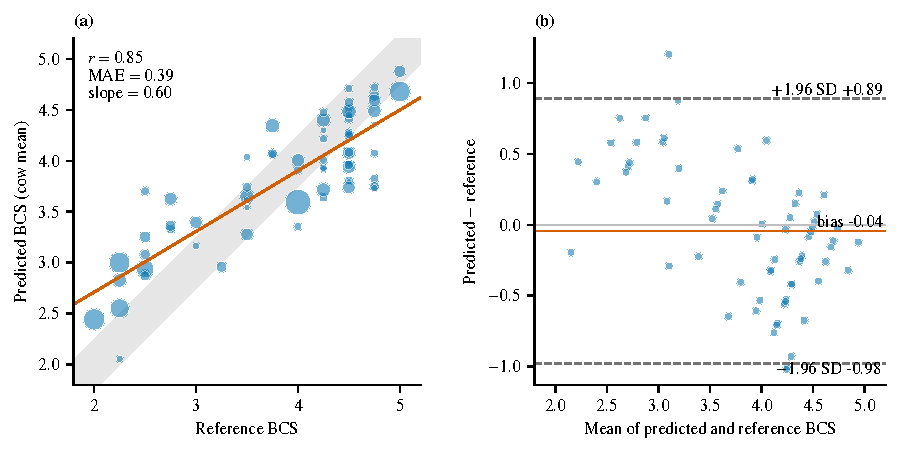
\includegraphics[width=\textwidth]{../figures/analisis_bland_altman.pdf}
  \caption{Agreement with the reference score (leave-one-cow-out; one point per cow and score, size proportional to the number of images). (a) Predicted against reference BCS; dashed: identity, grey band: $\pm0.25$, orange: least-squares fit. (b) Bland--Altman plot; orange: mean difference, dashed: 95\% limits of agreement.}
  \label{fig:ba}
\end{figure*}

\subsection{Stability over time and sample size}

Predictions for a given cow were stable from day to day.
For the 55 cow--score pairs photographed on at least two days, the daily mean prediction varied with a median SD of 0.23 points, less than the typical bias of each cow (0.42), and 86\% of the variance of the predictions lay between cows (intraclass correlation 0.86).
The error is therefore mostly a stable offset per cow rather than noise between photos, which is also why averaging more photos of the same cow helps little.
The model also followed real changes in condition (Fig.~\ref{fig:tracking}).
Cow 9008 fell ill and was rescored from 4.5 to 2.25 within a month; her predictions dropped from 4.15 at the start of the period to about 3.0--3.4 in early June, while she was still recorded as 4.5, and to 2.0 when she was rescored.
Cow 8758, scored 4.25, 4.0 and 3.5 in three months, was predicted at 3.92, 4.01 and 3.54.

\begin{figure}[t]
  \centering
  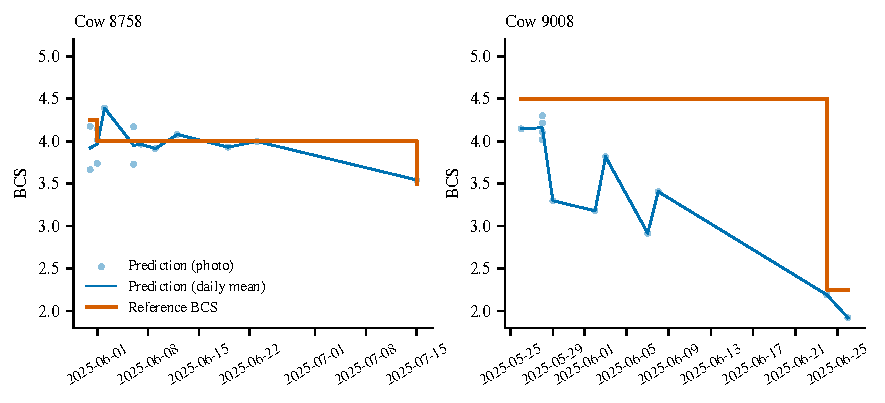
\includegraphics[width=\linewidth]{../figures/analisis_cambios_bcs.pdf}
  \caption{Predictions (leave-one-cow-out) for the two cows whose score changed during the study; orange: reference score.}
  \label{fig:tracking}
\end{figure}

Finally, the error kept falling as more cows were used for training: the MAE per cow went from 0.69 with 8 cows to 0.57 with 16, 0.48 with 32 and 0.44 with 56, while the bias for thin cows fell from +0.99 to +0.55.
A fit of the form $a + b/\sqrt{n}$ to the MAE per cow suggests about 0.40 with 100 cows and 0.37 with 200 (Fig.~\ref{fig:curve}), an extrapolation that assumes new cows resemble the present ones.

\begin{figure*}[t]
  \centering
  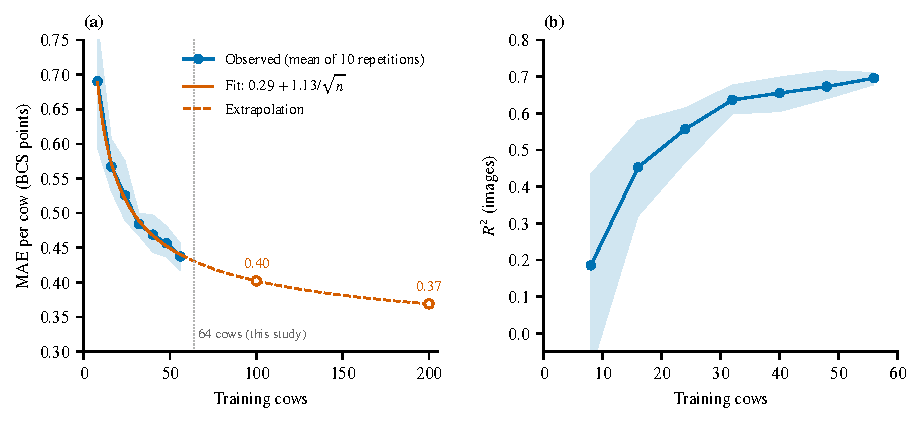
\includegraphics[width=\textwidth]{../figures/curva_aprendizaje.pdf}
  \caption{Learning curve. The model was trained on random subsets of $n$ cows and tested on eight held-out cows (8 folds $\times$ 10 repetitions). (a) MAE per cow; band: 2.5--97.5 percentiles over repetitions; orange: fit $a + b/\sqrt{n}$ and its extrapolation. (b) $R^2$ over images.}
  \label{fig:curve}
\end{figure*}
